\documentclass{article}

\usepackage{float}
\usepackage{graphicx}
\usepackage[margin=1in]{geometry}
\usepackage{amsmath}

\title{Hurricane Characterization with Common Inferential Statistics and Machine Learning Techniques}
\author{Charlie Edelson}
\date{}

\providecommand{\keywords}[1]{\small{\textit{Keywords:} #1}}


\begin{document}
	
	\maketitle

	% UPDATE ABSTRACT
	\begin{abstract}
	This is where the abstract will eventually go. However, currently we only have a place holder.
	\end{abstract}
	
	% UPDATE THE KEYWORKS!!!
	\keywords{word1, word2, word3}

	\section{Introduction}
	% UPDATE BACKGROUND HERE!!!!	
	The purpose of this paper is to investigate the properties of named storms in the Atlantic ocean basin using inferential 
statistics and machine learning techniques. Quadratic and Cubic polynomial regressions will be used to parameterize and model storm 
windspeed as a function of time, with coefficients binned across storms. ARIMA models will then be fit to each storm, and the most common 
models will be further investigated. Additionally, the average number of storms per year, $\lambda$, will be investigated using Bayesian 
statistics to get a distribution on probable values of $\lambda$. Finally, points in windspeed vs pressure phase space will be clustered 
using two classical machine learning technique, k means clustering and hierarchical clustering. These results will serve as a starting point for further investigation into storm characterization with statistical methods.

	Unisys 2000-2010 Hurricane/Tropical storm data was used throughout this paper\cite{Unisys}. This data consists of timestamped 
measurements of storm pressure, temperature, windspeed, latitude, and longitude for all major tropical depressions, tropical storms, and 
hurricanes between 2000 and 2010. Measurements were taken at approximately six hour intervals. Furthermore, storm name is included for all 
tropical storms and hurricanes.

	This data was selected for two reasons. The first is the data is consistent, with few missing time intervals. The second is the data tracks the storms directly. The research does not have to make a judgment call of which local sensors (buoy, ground station, etc.) are best representative of the storm at a given time and location. This increases the repeatability, since the original data does not need to be reinterpreted by each new investigator.

	\section{Methods}	 
	 Unnamed storms were removed from the data, as they are not the focus of this study, leaving 157 named storms over the 10 year period. 

	\subsection{Polynomial Regression}
	To understand the general shape of the windspeed profile, quadratic and cubic regression of the following forms
	
		\begin{align}
			w_i = \beta_0 + \beta_1 t_i + \beta_2 t_i^2\\
			w_i = \beta_0 + \beta_1 t_i + \beta_2 t_i^2 + \beta_3 t_i^3,
		\end{align}
	where $w_i$ is the windspeed at time $t_i$, were fit to each storm. The resulting coefficients, $\hat{\beta_i}$, were then binned 
according to values to create empirical distribution.

	\subsection{ARIMA Modeling}
	Each storm was cast into a time series and missing time steps were linearly interpolated. The minimum AIC ARIMA was then computed for $p, q, d \le 3$. The order tuple was recorded and tallied for each unique occurrence.

	\subsection{Estimation of $\lambda$}
	Since named storms are an example of a poisson process, an estimate of the shape parameter $\lambda$, the average number of storms per year, can be computed using Bayesian analysis. The likelihood function for the evidence $D$ given $\lambda$ would then be
	
		\begin{equation}
			P(D | \lambda) = \frac{\lambda^k e^{-n \lambda}}{k!},
		\end{equation}
		where $k$ is the number of storms observed in $n$ years. It is well known that the gamma distribution, $Gamma(\alpha, \beta)$, is a conjugate prior for the poisson distribution, where $\alpha$ and $\beta$ are the shape and inverse scale parameter, respectively. Therefore, given a gamma prior, with appropriate initial shape and inverse scale parameters, we can compute the posterior distribution as
		
		\begin{equation}
			P(\lambda | D) = Gamma(\alpha + k, \beta + n).
		\end{equation}
		

	\subsection{Cluster Analysis of Pressure and Wind Speed}
	Observed points were plotted in pressure vs wind speed phase space and then clustered using two common machine learning technique: k means clustering and hierarchical clustering. To compare results to the Saffir-Simpson scale\cite{}, 6 clusters were selected in both cases.

	\section{Analysis and Results}
		 All computational analysis was performed using the python programming language with the Pandas, Scipy, NumPy, Scikit-Learn, and Stats-Models libraries\cite{mckinney2010data, scipy, walt2011numpy, scikit-learn, statsmodels2010}. Graphics and visualizations were created using the Matplotlib and Seaborn libraries\cite{hunter2007matplotlib, michael_waskom_2014_12710}.
		 
	\subsection{Polynomial Regression}
	In both the quadratic and cubic regressions the constant coefficient dominates the model (Fig. \ref{quadratic} and \ref{cubic}). This indicates the shape of a storm's wind profile is not representable as a polynomial of low degree. Although a higher degree polynomial could be used, reducing model variance, this would increase model bias. Aside from the risk of overfitting, a higher degree polynomial has no clear interpretation in the given context.

	\begin{figure}[H]
			\centering
			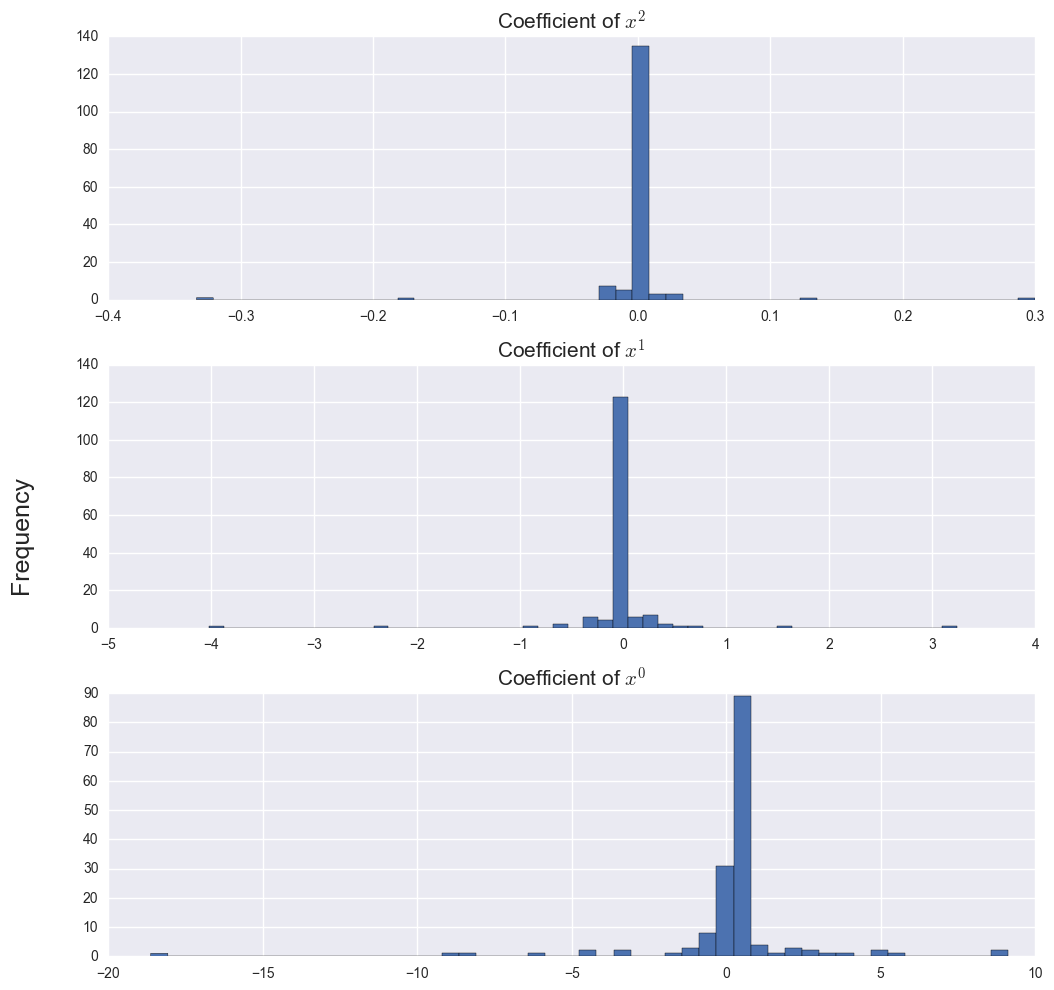
\includegraphics[width=0.55\textwidth]{images/quadratic.png}
		\caption{Histograms of the coefficients for the quadratic models fitted to each storm. Notice that $\hat{\beta_1}$ and $\hat{\beta_2}$ are both centered near zero. $\hat{\beta_0}$ has a much larger range, and is shifted slightly in the positive direction, indicating the constant coefficient dominated most models.}
		\label{quadratic}
	\end{figure}
	
	\begin{figure}[H]
			\centering
			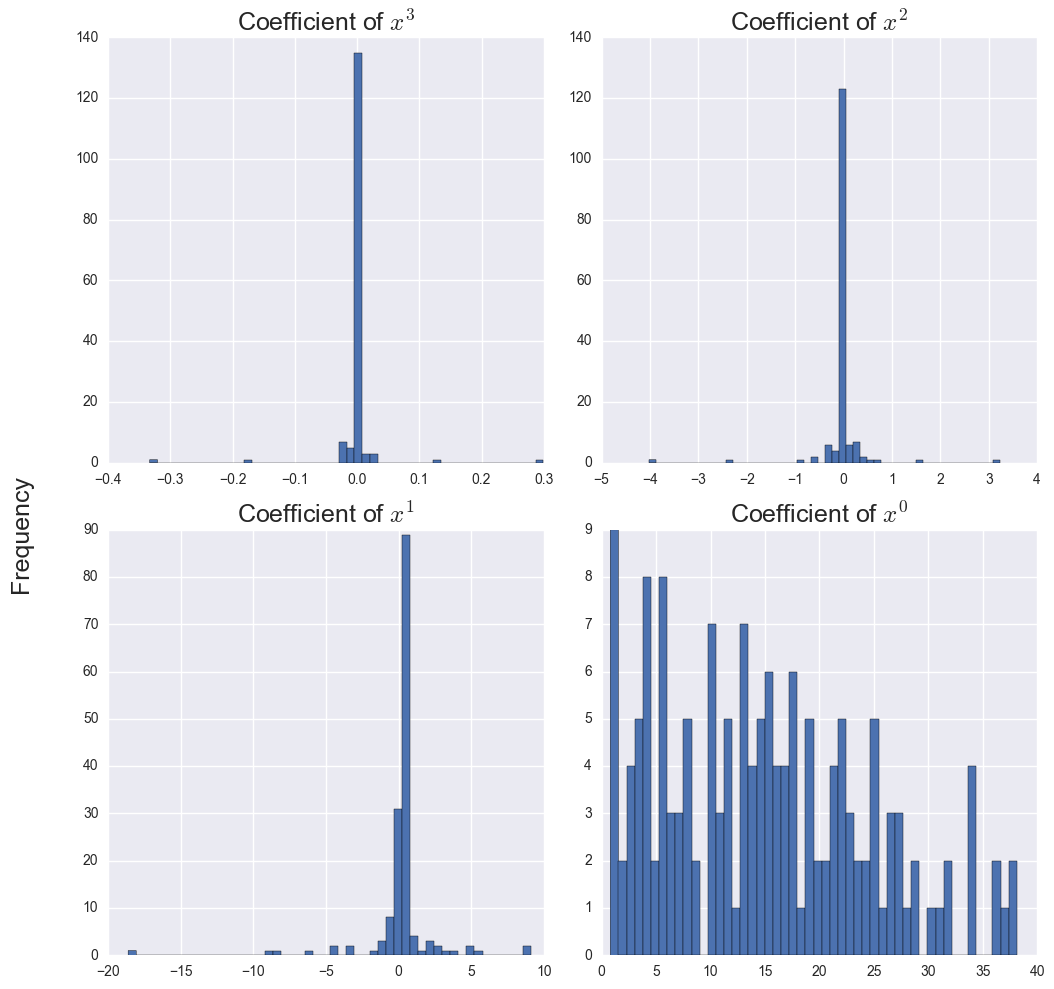
\includegraphics[width=0.55\textwidth]{images/cubic.png}
		\caption{Histograms of the coefficients for the cubic models fitted to each storm. Notice that the first coefficient for $x_1$, $x_2$, and $x_3$ are all centered around zero, while $x_0$ has a much larger range and many more non-zero values. This indicates -- as in the quadratic model -- the constant coefficient is dominating the model.}
		\label{cubic}
	\end{figure}

	\subsection{ARIMA Model}
	For the 157 storms, an order tuple of $(0,2,1)$ showed up more consistently than any other option (Fig. \ref{arima}). A differencing of $d=2$ is seen in eight of the ten top models, indicating a quadratic trend in windspeed. Furthermore, $q=1$ and $p=0$ suggests that the storm depending on only the previous time step with zero autocorrelation.
	
	\begin{figure}[t]
			\centering
			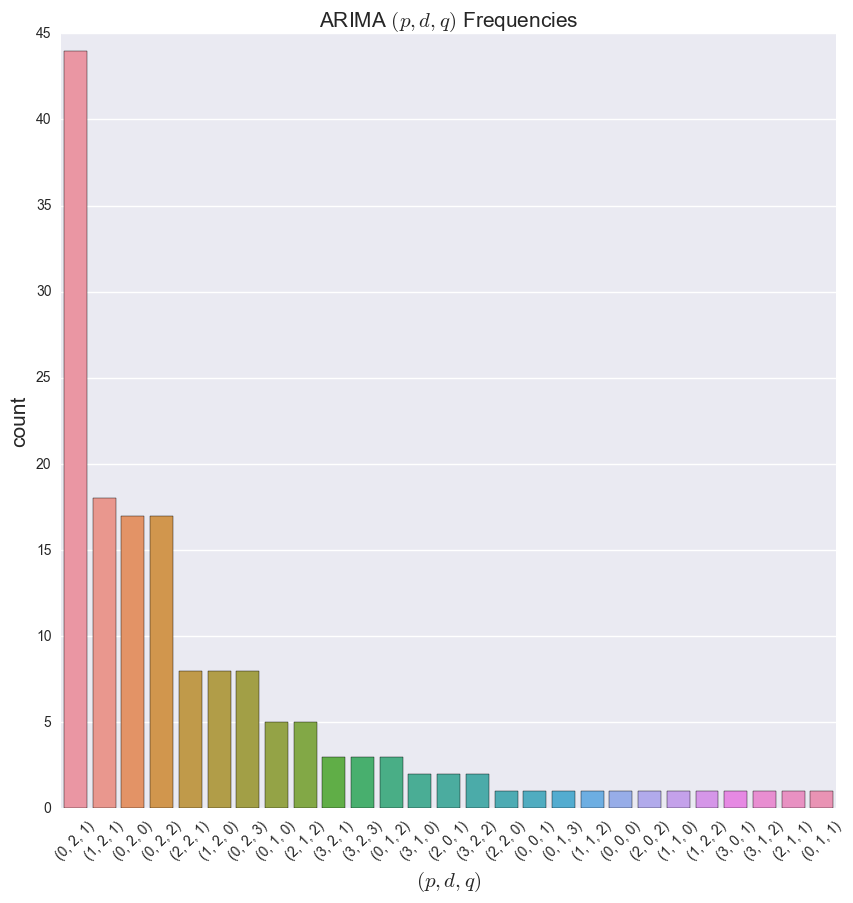
\includegraphics[width=0.55\textwidth]{images/arima.png}
		\caption{Count plot for the minimum AIC ARIMA coefficient for the 157 named storms. The $(0,2,1)$ model appears far more often than any other model. Additionally, a differencing of $d = 2$ appears in the top seven models.}
		\label{arima}
	\end{figure}

	\subsection{Bayesian Estimation of $\lambda$}
	The prior distribution is given by $Gamma(\alpha = 2, \beta = 1/12)$, and is plotted in Fig. \ref{prior}. This choice of parameters creates large wide spike with a mode of 12, which is what the author believe to be the most likely value of $\lambda$.
	
	

	
	\bibliography{sources}
	\bibliographystyle{ieeetr}

\end{document}
